%%%%%%%%%%%%%%%%%%%%%%%%%%%%%%%%%%%%%%%%%%%%%%%%%%%%%%%%%%%%%%%%%%%%%%%%%%%%%%%%
% Jag skall festa
%%%%%%%%%%%%%%%%%%%%%%%%%%%%%%%%%%%%%%%%%%%%%%%%%%%%%%%%%%%%%%%%%%%%%%%%%%%%%%%%

\settowidth{\versewidth}{Inte krypa runt med festeliten,}

\poemtitle{Jag skall festa}

%------------------------------------------------

\begin{verse}[\versewidth]

\flagverse{}
\emph{Mel. Bamse-låten}\\!

\flagverse{1.}
Jag skall festa, ta det lugnt med spriten,\\*
ha det roligt utan att va' full.\\*
Inte krypa runt med festeliten,\\*
ta det sansat för min egen skull.\\!

%------------------------------------------------

\flagverse{Refr.}
Först en öl i torra strupen,\\*
efter det så kommer supen,\\*
i med vinet, ned med punschen\\*
sist en groggbuffé\\!

%------------------------------------------------

\flagverse{2.}
Jag är skitfull, däckar först av alla,\\*
missar festen, men vad gör väl de'.\\*
Blandar hejdlöst öl ch gammal filmjölk,\\*
kastar upp på bordsdamen bredve'.\\!

%------------------------------------------------

\flagverse{Refr.}
Först en öl i torra strupen...\\!

%------------------------------------------------

\begin{figure}[H]
    \centering
    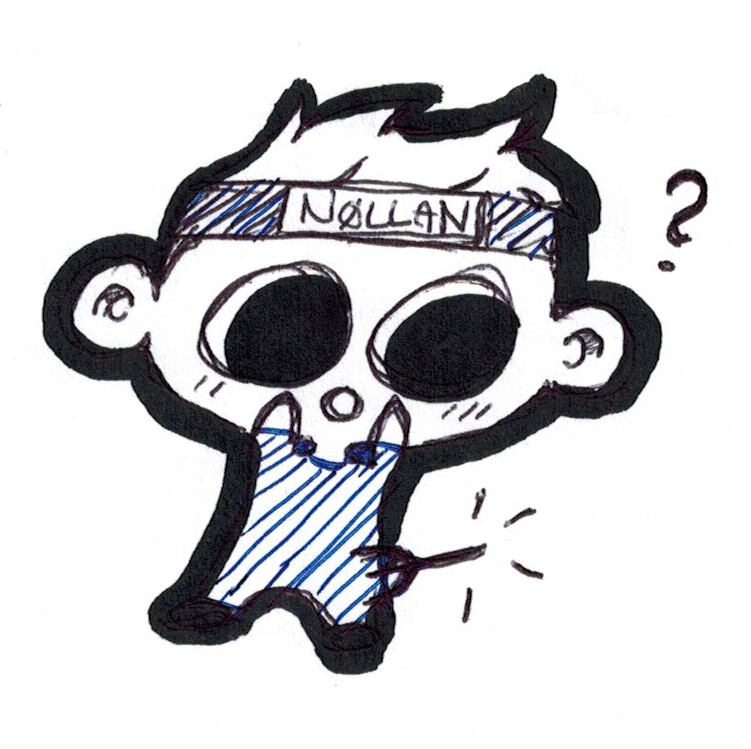
\includegraphics[width=0.5\textwidth]{nollan_ben.png}
\end{figure}

%------------------------------------------------

\flagverse{4.}
Spyan rinner ner för ylleslipsen,\\*
raviolin torkar i mitt hår.\\*
Vem har lagt mig här i pissoaren,\\*
vems är gaffeln i mitt högra lår?\\!

%------------------------------------------------

\flagverse{Refr.}
Först en öl i torra strupen...\\!

%------------------------------------------------

\poemauthorcenter{D-LTH, sångarstriden 1987}

%------------------------------------------------

\end{verse}

%----------------------------------------------------------------------------------------